% Options for packages loaded elsewhere
\PassOptionsToPackage{unicode}{hyperref}
\PassOptionsToPackage{hyphens}{url}
\PassOptionsToPackage{dvipsnames,svgnames,x11names}{xcolor}
%
\documentclass[
]{report}

\usepackage{amsmath,amssymb}
\usepackage{iftex}
\ifPDFTeX
  \usepackage[T1]{fontenc}
  \usepackage[utf8]{inputenc}
  \usepackage{textcomp} % provide euro and other symbols
\else % if luatex or xetex
  \usepackage{unicode-math}
  \defaultfontfeatures{Scale=MatchLowercase}
  \defaultfontfeatures[\rmfamily]{Ligatures=TeX,Scale=1}
\fi
\usepackage{lmodern}
\ifPDFTeX\else  
    % xetex/luatex font selection
\fi
% Use upquote if available, for straight quotes in verbatim environments
\IfFileExists{upquote.sty}{\usepackage{upquote}}{}
\IfFileExists{microtype.sty}{% use microtype if available
  \usepackage[]{microtype}
  \UseMicrotypeSet[protrusion]{basicmath} % disable protrusion for tt fonts
}{}
\makeatletter
\@ifundefined{KOMAClassName}{% if non-KOMA class
  \IfFileExists{parskip.sty}{%
    \usepackage{parskip}
  }{% else
    \setlength{\parindent}{0pt}
    \setlength{\parskip}{6pt plus 2pt minus 1pt}}
}{% if KOMA class
  \KOMAoptions{parskip=half}}
\makeatother
\usepackage{xcolor}
\setlength{\emergencystretch}{3em} % prevent overfull lines
\setcounter{secnumdepth}{-\maxdimen} % remove section numbering
% Make \paragraph and \subparagraph free-standing
\makeatletter
\ifx\paragraph\undefined\else
  \let\oldparagraph\paragraph
  \renewcommand{\paragraph}{
    \@ifstar
      \xxxParagraphStar
      \xxxParagraphNoStar
  }
  \newcommand{\xxxParagraphStar}[1]{\oldparagraph*{#1}\mbox{}}
  \newcommand{\xxxParagraphNoStar}[1]{\oldparagraph{#1}\mbox{}}
\fi
\ifx\subparagraph\undefined\else
  \let\oldsubparagraph\subparagraph
  \renewcommand{\subparagraph}{
    \@ifstar
      \xxxSubParagraphStar
      \xxxSubParagraphNoStar
  }
  \newcommand{\xxxSubParagraphStar}[1]{\oldsubparagraph*{#1}\mbox{}}
  \newcommand{\xxxSubParagraphNoStar}[1]{\oldsubparagraph{#1}\mbox{}}
\fi
\makeatother

\usepackage{color}
\usepackage{fancyvrb}
\newcommand{\VerbBar}{|}
\newcommand{\VERB}{\Verb[commandchars=\\\{\}]}
\DefineVerbatimEnvironment{Highlighting}{Verbatim}{commandchars=\\\{\}}
% Add ',fontsize=\small' for more characters per line
\usepackage{framed}
\definecolor{shadecolor}{RGB}{241,243,245}
\newenvironment{Shaded}{\begin{snugshade}}{\end{snugshade}}
\newcommand{\AlertTok}[1]{\textcolor[rgb]{0.68,0.00,0.00}{#1}}
\newcommand{\AnnotationTok}[1]{\textcolor[rgb]{0.37,0.37,0.37}{#1}}
\newcommand{\AttributeTok}[1]{\textcolor[rgb]{0.40,0.45,0.13}{#1}}
\newcommand{\BaseNTok}[1]{\textcolor[rgb]{0.68,0.00,0.00}{#1}}
\newcommand{\BuiltInTok}[1]{\textcolor[rgb]{0.00,0.23,0.31}{#1}}
\newcommand{\CharTok}[1]{\textcolor[rgb]{0.13,0.47,0.30}{#1}}
\newcommand{\CommentTok}[1]{\textcolor[rgb]{0.37,0.37,0.37}{#1}}
\newcommand{\CommentVarTok}[1]{\textcolor[rgb]{0.37,0.37,0.37}{\textit{#1}}}
\newcommand{\ConstantTok}[1]{\textcolor[rgb]{0.56,0.35,0.01}{#1}}
\newcommand{\ControlFlowTok}[1]{\textcolor[rgb]{0.00,0.23,0.31}{\textbf{#1}}}
\newcommand{\DataTypeTok}[1]{\textcolor[rgb]{0.68,0.00,0.00}{#1}}
\newcommand{\DecValTok}[1]{\textcolor[rgb]{0.68,0.00,0.00}{#1}}
\newcommand{\DocumentationTok}[1]{\textcolor[rgb]{0.37,0.37,0.37}{\textit{#1}}}
\newcommand{\ErrorTok}[1]{\textcolor[rgb]{0.68,0.00,0.00}{#1}}
\newcommand{\ExtensionTok}[1]{\textcolor[rgb]{0.00,0.23,0.31}{#1}}
\newcommand{\FloatTok}[1]{\textcolor[rgb]{0.68,0.00,0.00}{#1}}
\newcommand{\FunctionTok}[1]{\textcolor[rgb]{0.28,0.35,0.67}{#1}}
\newcommand{\ImportTok}[1]{\textcolor[rgb]{0.00,0.46,0.62}{#1}}
\newcommand{\InformationTok}[1]{\textcolor[rgb]{0.37,0.37,0.37}{#1}}
\newcommand{\KeywordTok}[1]{\textcolor[rgb]{0.00,0.23,0.31}{\textbf{#1}}}
\newcommand{\NormalTok}[1]{\textcolor[rgb]{0.00,0.23,0.31}{#1}}
\newcommand{\OperatorTok}[1]{\textcolor[rgb]{0.37,0.37,0.37}{#1}}
\newcommand{\OtherTok}[1]{\textcolor[rgb]{0.00,0.23,0.31}{#1}}
\newcommand{\PreprocessorTok}[1]{\textcolor[rgb]{0.68,0.00,0.00}{#1}}
\newcommand{\RegionMarkerTok}[1]{\textcolor[rgb]{0.00,0.23,0.31}{#1}}
\newcommand{\SpecialCharTok}[1]{\textcolor[rgb]{0.37,0.37,0.37}{#1}}
\newcommand{\SpecialStringTok}[1]{\textcolor[rgb]{0.13,0.47,0.30}{#1}}
\newcommand{\StringTok}[1]{\textcolor[rgb]{0.13,0.47,0.30}{#1}}
\newcommand{\VariableTok}[1]{\textcolor[rgb]{0.07,0.07,0.07}{#1}}
\newcommand{\VerbatimStringTok}[1]{\textcolor[rgb]{0.13,0.47,0.30}{#1}}
\newcommand{\WarningTok}[1]{\textcolor[rgb]{0.37,0.37,0.37}{\textit{#1}}}

\providecommand{\tightlist}{%
  \setlength{\itemsep}{0pt}\setlength{\parskip}{0pt}}\usepackage{longtable,booktabs,array}
\usepackage{calc} % for calculating minipage widths
% Correct order of tables after \paragraph or \subparagraph
\usepackage{etoolbox}
\makeatletter
\patchcmd\longtable{\par}{\if@noskipsec\mbox{}\fi\par}{}{}
\makeatother
% Allow footnotes in longtable head/foot
\IfFileExists{footnotehyper.sty}{\usepackage{footnotehyper}}{\usepackage{footnote}}
\makesavenoteenv{longtable}
\usepackage{graphicx}
\makeatletter
\newsavebox\pandoc@box
\newcommand*\pandocbounded[1]{% scales image to fit in text height/width
  \sbox\pandoc@box{#1}%
  \Gscale@div\@tempa{\textheight}{\dimexpr\ht\pandoc@box+\dp\pandoc@box\relax}%
  \Gscale@div\@tempb{\linewidth}{\wd\pandoc@box}%
  \ifdim\@tempb\p@<\@tempa\p@\let\@tempa\@tempb\fi% select the smaller of both
  \ifdim\@tempa\p@<\p@\scalebox{\@tempa}{\usebox\pandoc@box}%
  \else\usebox{\pandoc@box}%
  \fi%
}
% Set default figure placement to htbp
\def\fps@figure{htbp}
\makeatother

\makeatletter
\@ifpackageloaded{caption}{}{\usepackage{caption}}
\AtBeginDocument{%
\ifdefined\contentsname
  \renewcommand*\contentsname{Table of contents}
\else
  \newcommand\contentsname{Table of contents}
\fi
\ifdefined\listfigurename
  \renewcommand*\listfigurename{List of Figures}
\else
  \newcommand\listfigurename{List of Figures}
\fi
\ifdefined\listtablename
  \renewcommand*\listtablename{List of Tables}
\else
  \newcommand\listtablename{List of Tables}
\fi
\ifdefined\figurename
  \renewcommand*\figurename{Figure}
\else
  \newcommand\figurename{Figure}
\fi
\ifdefined\tablename
  \renewcommand*\tablename{Table}
\else
  \newcommand\tablename{Table}
\fi
}
\@ifpackageloaded{float}{}{\usepackage{float}}
\floatstyle{ruled}
\@ifundefined{c@chapter}{\newfloat{codelisting}{h}{lop}}{\newfloat{codelisting}{h}{lop}[chapter]}
\floatname{codelisting}{Listing}
\newcommand*\listoflistings{\listof{codelisting}{List of Listings}}
\makeatother
\makeatletter
\makeatother
\makeatletter
\@ifpackageloaded{caption}{}{\usepackage{caption}}
\@ifpackageloaded{subcaption}{}{\usepackage{subcaption}}
\makeatother

\usepackage{bookmark}

\IfFileExists{xurl.sty}{\usepackage{xurl}}{} % add URL line breaks if available
\urlstyle{same} % disable monospaced font for URLs
\hypersetup{
  pdftitle={Database Course},
  pdfauthor={Lotfi NAJDI},
  colorlinks=true,
  linkcolor={blue},
  filecolor={Maroon},
  citecolor={Blue},
  urlcolor={Blue},
  pdfcreator={LaTeX via pandoc}}


\title{Database Course}
\usepackage{etoolbox}
\makeatletter
\providecommand{\subtitle}[1]{% add subtitle to \maketitle
  \apptocmd{\@title}{\par {\large #1 \par}}{}{}
}
\makeatother
\subtitle{Indexes for Speeding Up Queries}
\author{Lotfi NAJDI}
\date{}

\begin{document}
\maketitle


\section{What is a Database Index?}\label{what-is-a-database-index}

An index is a \textbf{data structure} that improves the speed of data
retrieval operations.

This is another object in the database that references the data in
tables.

\emph{Indexes speed up SELECT queries but slow down
INSERT/UPDATE/DELETE}

\begin{center}\rule{0.5\linewidth}{0.5pt}\end{center}

\section{A Simple Analogy 📚}\label{a-simple-analogy}

Think of an index as the \textbf{index} at the back of a book.

\begin{itemize}
\tightlist
\item
  Without an index: You'd have to read every page to find a topic
\item
  With an index: You jump directly to the page number
\item
  Database without index: Scans every row (FULL TABLE SCAN)
\item
  Database with index: Jumps directly to matching rows
\end{itemize}

\begin{center}\rule{0.5\linewidth}{0.5pt}\end{center}

\section{So, Why Use Indexes? 🚀}\label{so-why-use-indexes}

Indexes are essential for improving database performance:

\begin{itemize}
\tightlist
\item
  \textbf{Faster Query Performance}: Significantly reduces the time
  taken to retrieve data.
\end{itemize}

\begin{itemize}
\tightlist
\item
  \textbf{Efficient Data Access}: Optimizes search operations,
  especially on large datasets.
\end{itemize}

\begin{itemize}
\tightlist
\item
  \textbf{Reduced I/O Operations}: Minimizes the amount of data read
  from disk.
\end{itemize}

\begin{itemize}
\tightlist
\item
  \textbf{Improved Join Performance}: Speeds up join operations between
  tables.
\end{itemize}

\begin{center}\rule{0.5\linewidth}{0.5pt}\end{center}

\section{Full Table Scan}\label{full-table-scan}

\includegraphics[width=0.8\linewidth,height=\textheight,keepaspectratio]{images/full-scan.png}

\begin{itemize}
\tightlist
\item
  This is a Full Table Scan.
\item
  Databases do this by default.
\item
  It's a huge performance bottleneck for large tables.
\end{itemize}

\begin{center}\rule{0.5\linewidth}{0.5pt}\end{center}

\section{Performance Cost: Linear
Growth}\label{performance-cost-linear-growth}

\includegraphics[width=1\linewidth,height=\textheight,keepaspectratio]{images/o1-full-scan.png}

\begin{itemize}
\tightlist
\item
  Full Table Scan performance is directly proportional to table size
\item
  O(N) complexity
\item
  Double the data = double the wait time
\item
  Linear scaling is the enemy of fast applications
\end{itemize}

\section{The Solution: The Database
Index}\label{the-solution-the-database-index}

\pandocbounded{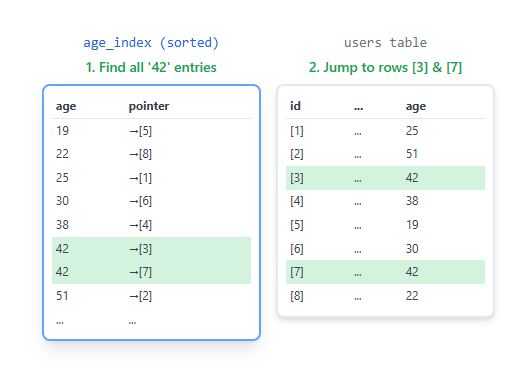
\includegraphics[keepaspectratio]{images/solution-index.png}}

\begin{itemize}
\tightlist
\item
  An index is like a book's index: a separate, sorted structure that
  points directly to the data's location.
\item
  Instead of scanning the whole table, RDBMS uses the index to find all
  matching rows instantly.
\end{itemize}

\begin{center}\rule{0.5\linewidth}{0.5pt}\end{center}

\section{Performance Gain: Logarithmic
Growth}\label{performance-gain-logarithmic-growth}

\includegraphics[width=0.8\linewidth,height=\textheight,keepaspectratio]{images/o-log-scan.png}

\begin{itemize}
\tightlist
\item
  An Index Scan's performance barely changes, even when the table grows
  exponentially.
\item
  This is O(log N) complexity.
\item
  The magic of an index: Ten times the data might not even add a
  millisecond to your query.
\item
  This is why indexes are critical for scaling.
\end{itemize}

\begin{center}\rule{0.5\linewidth}{0.5pt}\end{center}

\section{The Golden Trade-Off}\label{the-golden-trade-off}

Indexes are not free. They create a fundamental trade-off.

\begin{itemize}
\tightlist
\item
  \textbf{FASTER Reads (SELECT)}: Queries on indexed columns are
  dramatically faster.
\item
  \textbf{SLOWER Writes (INSERT, UPDATE, DELETE)}: Postgres must do
  extra work to update the index too.
\end{itemize}

\chapter{How Indexes Work Internally}\label{how-indexes-work-internally}

\section{Physical Storage of Indexes}\label{physical-storage-of-indexes}

Indexes are stored as \textbf{separate data structures} on disk,
independent of the table data.

Each index occupies its own space and requires maintenance on every data
modification.

PostgreSQL uses \textbf{pages} (8KB blocks) to store both table data and
index data.

\begin{center}\rule{0.5\linewidth}{0.5pt}\end{center}

\section{B-Tree Index Structure 🌳}\label{b-tree-index-structure}

\textbf{B-Tree} (Balanced Tree) is the default and most versatile index
type in PostgreSQL.

\section{The Structure of an Index: The
B-Tree}\label{the-structure-of-an-index-the-b-tree}

\includegraphics[width=0.8\linewidth,height=\textheight,keepaspectratio]{images/btree-structure.png}

\begin{itemize}
\tightlist
\item
  \textbf{Root Node}: Entry point
\item
  \textbf{Internal Nodes}: Navigation
\item
  \textbf{Leaf Nodes}: Point to data
\end{itemize}

\begin{center}\rule{0.5\linewidth}{0.5pt}\end{center}

\section{B-Tree search}\label{b-tree-search}

\includegraphics[width=0.8\linewidth,height=\textheight,keepaspectratio]{images/b-tree-search.png}

\begin{itemize}
\tightlist
\item
  Keys are always kept in sorted order within each node.
\item
  This allows for incredibly fast searching.
\item
  Just like finding a word in a dictionary, the database can make a
  quick decision at each step to narrow down the search.
\end{itemize}

\begin{center}\rule{0.5\linewidth}{0.5pt}\end{center}

\section{How B-Tree Search Works}\label{how-b-tree-search-works}

\begin{enumerate}
\def\labelenumi{\arabic{enumi}.}
\tightlist
\item
  \textbf{Start at Root}: Compare search value with root node
\item
  \textbf{Navigate Down}: Follow pointer to appropriate child node
\item
  \textbf{Repeat}: Continue until reaching leaf node
\item
  \textbf{Find Data}: Leaf node contains pointer to actual table row
\end{enumerate}

\subsection{Example: Finding value 30}\label{example-finding-value-30}

\begin{Shaded}
\begin{Highlighting}[]
\NormalTok{Root (50) → Go Left → Internal (25) → Go Right → Leaf [26{-}49]}
\end{Highlighting}
\end{Shaded}

\subsection{Example: Finding value 80}\label{example-finding-value-80}

\begin{Shaded}
\begin{Highlighting}[]
\NormalTok{Root (50) → Go Right → Internal (75) → Go Right → Leaf [76{-}100]}
\end{Highlighting}
\end{Shaded}

\section{B-Tree Page Structure}\label{b-tree-page-structure}

Each node is stored in one or more \textbf{pages}:

\begin{Shaded}
\begin{Highlighting}[]
\NormalTok{┌──────────────────────┐}
\NormalTok{│   Page               │}
\NormalTok{├──────────────────────┤}
\NormalTok{│   Index Tuples       │}
\NormalTok{│   (Key + Pointer)    │}
\NormalTok{└──────────────────────┘}
\end{Highlighting}
\end{Shaded}

\begin{itemize}
\tightlist
\item
  \textbf{Keys}: contain the indexed column values like 1, 25, 50, 75
\item
  \textbf{Pointers}: point to child nodes or actual table rows
\end{itemize}

\begin{center}\rule{0.5\linewidth}{0.5pt}\end{center}

\section{B-Tree Leaf Nodes}\label{b-tree-leaf-nodes}

Leaf nodes contain the actual pointers to the table rows.

\begin{Shaded}
\begin{Highlighting}[]
\NormalTok{┌─────────────────────────────┐}
\NormalTok{│   Leaf Page                 │}
\NormalTok{├─────────────────────────────┤}
\NormalTok{│   Key: 1   → Pointer to Row │}
\NormalTok{│   Key: 2   → Pointer to Row │}
\NormalTok{│   Key: 3   → Pointer to Row │}
\NormalTok{│   ...                       │}
\NormalTok{│   Key: 100 → Pointer to Row │}
\NormalTok{└─────────────────────────────┘}
\end{Highlighting}
\end{Shaded}

\chapter{Creating and Verifying
Indexe}\label{creating-and-verifying-indexe}

\section{Single Column Index}\label{single-column-index}

The SQL syntax for creating an index is straightforward. A common naming
convention is \texttt{idx\_tablename\_columnname}.

\begin{Shaded}
\begin{Highlighting}[]
\CommentTok{{-}{-} For a single column:}
\KeywordTok{CREATE} \KeywordTok{INDEX}\NormalTok{ idx\_users\_username }
\KeywordTok{ON}\NormalTok{ users (username);}
\end{Highlighting}
\end{Shaded}

\section{Confirm index creation}\label{confirm-index-creation}

\begin{Shaded}
\begin{Highlighting}[]
\KeywordTok{SELECT}\NormalTok{ indexname, indexdef }
\KeywordTok{FROM}\NormalTok{ pg\_indexes }
\KeywordTok{WHERE}\NormalTok{ tablename }\OperatorTok{=} \StringTok{\textquotesingle{}users\textquotesingle{}}\NormalTok{;}
\end{Highlighting}
\end{Shaded}

\textbf{Expected Output:}

\begin{Shaded}
\begin{Highlighting}[]
\NormalTok{indexname                     | indexdef}
\NormalTok{{-}{-}{-}{-}{-}{-}{-}{-}{-}{-}{-}{-}{-}{-}{-}{-}{-}{-}{-}{-}{-}{-}{-}{-}{-}{-}{-}{-}{-}{-}|{-}{-}{-}{-}{-}{-}{-}{-}{-}{-}{-}{-}{-}{-}{-}{-}{-}{-}{-}{-}{-}{-}{-}{-}{-}{-}{-}{-}{-}{-}{-}{-}{-}{-}{-}{-}{-}{-}{-}{-}{-}{-}}
\NormalTok{users\_pkey                    | CREATE UNIQUE INDEX users\_pkey ON users USING btree (id)}
\NormalTok{idx\_users\_username            | CREATE INDEX idx\_users\_username ON users USING btree (username)}
\end{Highlighting}
\end{Shaded}

\d users allows you to view the table structure and all indexes
associated with the users table.

\section{Primary Keys - Automatic
Index}\label{primary-keys---automatic-index}

PostgreSQL automatically creates a \textbf{unique B-tree index} on
primary key columns. For foreign keys and relationships, \textbf{indexes
are essential but not automatic}.

\section{Multi-Column (Composite)
Indexes}\label{multi-column-composite-indexes}

You can index multiple columns for queries that filter on several fields
at once.

\begin{Shaded}
\begin{Highlighting}[]
\KeywordTok{CREATE} \KeywordTok{INDEX}\NormalTok{ idx\_users\_fullname }
\KeywordTok{ON}\NormalTok{ users (first\_name, last\_name);}
\end{Highlighting}
\end{Shaded}

Important: The order of columns matters!
\texttt{(last\_name,\ first\_name)} is not the same as
\texttt{(first\_name,\ last\_name)}.

\section{Confirm Composite Index
Creation}\label{confirm-composite-index-creation}

\begin{Shaded}
\begin{Highlighting}[]
\KeywordTok{SELECT}\NormalTok{ indexname, indexdef }
\KeywordTok{FROM}\NormalTok{ pg\_indexes }
\KeywordTok{WHERE}\NormalTok{ tablename }\OperatorTok{=} \StringTok{\textquotesingle{}users\textquotesingle{}}\NormalTok{;}
\end{Highlighting}
\end{Shaded}

\textbf{Expected Output:}

\begin{Shaded}
\begin{Highlighting}[]
\NormalTok{indexname                     | indexdef}
\NormalTok{{-}{-}{-}{-}{-}{-}{-}{-}{-}{-}{-}{-}{-}{-}{-}{-}{-}{-}{-}{-}{-}{-}{-}{-}{-}{-}{-}{-}{-}{-}|{-}{-}{-}{-}{-}{-}{-}{-}{-}{-}{-}{-}{-}{-}{-}{-}{-}{-}{-}{-}{-}{-}{-}{-}{-}{-}{-}{-}{-}{-}{-}{-}{-}{-}{-}{-}{-}{-}{-}{-}{-}{-}}
\NormalTok{users\_pkey                    | CREATE UNIQUE INDEX users\_pkey ON users USING btree (id)}
\NormalTok{idx\_users\_username            | CREATE INDEX idx\_users\_username ON users USING btree (username)}
\NormalTok{idx\_users\_fullname            | CREATE INDEX idx\_users\_fullname ON users USING btree (first\_name, last\_name)}
\end{Highlighting}
\end{Shaded}

\section{Dropping Index}\label{dropping-index}

\begin{Shaded}
\begin{Highlighting}[]
\KeywordTok{DROP} \KeywordTok{INDEX}\NormalTok{ index\_name;}
\end{Highlighting}
\end{Shaded}

\section{Index Maintenance}\label{index-maintenance}

\subsection{Dropping unused indexes}\label{dropping-unused-indexes}

\begin{Shaded}
\begin{Highlighting}[]
\CommentTok{{-}{-} Remove an index if it\textquotesingle{}s not being used}
\KeywordTok{DROP} \KeywordTok{INDEX}\NormalTok{ idx\_customer\_last\_name;}
\end{Highlighting}
\end{Shaded}

\subsection{Reindexing for
maintenance}\label{reindexing-for-maintenance}

\begin{Shaded}
\begin{Highlighting}[]
\CommentTok{{-}{-} Rebuild an index to optimize it}
\NormalTok{REINDEX }\KeywordTok{INDEX}\NormalTok{ idx\_customer\_last\_name;}

\CommentTok{{-}{-} Rebuild all indexes on a table}
\NormalTok{REINDEX }\KeywordTok{TABLE}\NormalTok{ customers;}
\end{Highlighting}
\end{Shaded}

\begin{center}\rule{0.5\linewidth}{0.5pt}\end{center}

\section{Unique Indexes}\label{unique-indexes}

\subsection{Enforcing data uniqueness}\label{enforcing-data-uniqueness}

\begin{Shaded}
\begin{Highlighting}[]
\CommentTok{{-}{-} Create unique index to prevent duplicate emails}
\KeywordTok{CREATE} \KeywordTok{UNIQUE} \KeywordTok{INDEX}\NormalTok{ idx\_customers\_email\_unique }
\KeywordTok{ON}\NormalTok{ customers (email);}

\CommentTok{{-}{-} This will fail if email already exists}
\KeywordTok{INSERT} \KeywordTok{INTO}\NormalTok{ customers (email, name) }
\KeywordTok{VALUES}\NormalTok{ (}\StringTok{\textquotesingle{}existing@email.com\textquotesingle{}}\NormalTok{, }\StringTok{\textquotesingle{}John Doe\textquotesingle{}}\NormalTok{);}
\end{Highlighting}
\end{Shaded}

\begin{center}\rule{0.5\linewidth}{0.5pt}\end{center}

\section{Performance Tips}\label{performance-tips}

\begin{itemize}
\tightlist
\item
  ✅ \textbf{Index foreign keys} - JOIN operations will be faster
\end{itemize}

\begin{itemize}
\tightlist
\item
  ✅ \textbf{Index WHERE clause columns} - Especially in frequent
  queries
\end{itemize}

\begin{itemize}
\tightlist
\item
  ✅ \textbf{Index ORDER BY columns} - Sorting will be faster
\end{itemize}

\begin{itemize}
\tightlist
\item
  ✅ \textbf{Monitor index usage} - Remove unused indexes
\end{itemize}

\begin{itemize}
\tightlist
\item
  ✅ \textbf{Consider composite indexes} - For multi-column WHERE
  clauses
\end{itemize}

\section{Real-World Example}\label{real-world-example}

\begin{Shaded}
\begin{Highlighting}[]
\CommentTok{{-}{-} Products table with proper indexes}
\KeywordTok{CREATE} \KeywordTok{TABLE}\NormalTok{ products (}
\NormalTok{    product\_id SERIAL }\KeywordTok{PRIMARY} \KeywordTok{KEY}\NormalTok{,  }\CommentTok{{-}{-} Automatic index}
\NormalTok{    name }\DataTypeTok{VARCHAR}\NormalTok{(}\DecValTok{255}\NormalTok{),}
\NormalTok{    category\_id }\DataTypeTok{INTEGER}\NormalTok{,}
\NormalTok{    price }\DataTypeTok{DECIMAL}\NormalTok{(}\DecValTok{10}\NormalTok{,}\DecValTok{2}\NormalTok{),}
\NormalTok{    created\_date }\DataTypeTok{DATE}\NormalTok{,}
\NormalTok{    status }\DataTypeTok{VARCHAR}\NormalTok{(}\DecValTok{20}\NormalTok{)}
\NormalTok{);}

\CommentTok{{-}{-} Strategic indexes}
\KeywordTok{CREATE} \KeywordTok{INDEX}\NormalTok{ idx\_products\_category }\KeywordTok{ON}\NormalTok{ products (category\_id);}
\KeywordTok{CREATE} \KeywordTok{INDEX}\NormalTok{ idx\_products\_price }\KeywordTok{ON}\NormalTok{ products (price);}
\KeywordTok{CREATE} \KeywordTok{INDEX}\NormalTok{ idx\_products\_status\_date }\KeywordTok{ON}\NormalTok{ products (status, created\_date);}
\end{Highlighting}
\end{Shaded}

\begin{center}\rule{0.5\linewidth}{0.5pt}\end{center}

\section{Common Mistakes to Avoid}\label{common-mistakes-to-avoid}

\begin{itemize}
\tightlist
\item
  🚫 \textbf{Creating too many indexes} - Slows down writes
\end{itemize}

\begin{itemize}
\tightlist
\item
  🚫 \textbf{Not monitoring index usage} - Wasted storage space
\end{itemize}

\begin{itemize}
\tightlist
\item
  🚫 \textbf{Wrong column order in composite indexes} - Put most
  selective column first
\end{itemize}

\begin{itemize}
\tightlist
\item
  🚫 \textbf{Indexing everything} - Each index has overhead
\end{itemize}

\chapter{Query Optimization}\label{query-optimization}

\section{The Explain Command}\label{the-explain-command}

\texttt{EXPLAIN} shows how PostgreSQL will execute a query - the
\textbf{query execution plan}.

\begin{Shaded}
\begin{Highlighting}[]
\KeywordTok{EXPLAIN}
\KeywordTok{SELECT} \OperatorTok{*} \KeywordTok{FROM}\NormalTok{ users }\KeywordTok{WHERE}\NormalTok{ username }\OperatorTok{=} \StringTok{\textquotesingle{}john\_doe\textquotesingle{}}\NormalTok{;}
\end{Highlighting}
\end{Shaded}

Expected Output:

\begin{Shaded}
\begin{Highlighting}[]
\NormalTok{                        QUERY PLAN}
\NormalTok{{-}{-}{-}{-}{-}{-}{-}{-}{-}{-}{-}{-}{-}{-}{-}{-}{-}{-}{-}{-}{-}{-}{-}{-}{-}{-}{-}{-}{-}{-}{-}{-}{-}{-}{-}{-}{-}{-}{-}{-}{-}{-}{-}{-}{-}{-}{-}{-}{-}{-}{-}{-}{-}{-}{-}{-}{-}{-}{-}}
\NormalTok{ Index Scan using idx\_users\_username on users  (cost=0.29..8.31}
\NormalTok{  rows=1 width=128)}
\NormalTok{    Index Cond: (username = \textquotesingle{}john\_doe\textquotesingle{})}
\NormalTok{(1 row)}
\end{Highlighting}
\end{Shaded}

\section{Anatomy of a Query Plan}\label{anatomy-of-a-query-plan}

\begin{Shaded}
\begin{Highlighting}[]
\NormalTok{                        QUERY PLAN}
\NormalTok{{-}{-}{-}{-}{-}{-}{-}{-}{-}{-}{-}{-}{-}{-}{-}{-}{-}{-}{-}{-}{-}{-}{-}{-}{-}{-}{-}{-}{-}{-}{-}{-}{-}{-}{-}{-}{-}{-}{-}{-}{-}{-}{-}{-}{-}{-}{-}{-}{-}{-}{-}{-}{-}{-}{-}{-}{-}{-}{-}}
\NormalTok{ Index Scan using idx\_users\_username on users  (cost=0.29..8.31}
\NormalTok{  rows=1 width=128)}
\NormalTok{    Index Cond: (username = \textquotesingle{}john\_doe\textquotesingle{})}
\NormalTok{(1 row)}
\end{Highlighting}
\end{Shaded}

Each line describes an operation. Let's break down the key parts:

\begin{itemize}
\tightlist
\item
  \textbf{Node Type}: The type of operation (e.g., Index Scan)
\item
  \textbf{Cost}: The planner's estimate of the work required

  \begin{itemize}
  \tightlist
  \item
    PostgreSQL doesn't measure cost in milliseconds --- it uses relative
    units so it can compare plans independently of hardware speed. Each
    action (CPU step, disk read, etc.) has a weight:
  \end{itemize}
\item
  \textbf{Rows}: The estimated number of rows this operation will return
\item
  \textbf{Width}: The average size (in bytes) of each row
\end{itemize}

\section{Decoding the `Cost'}\label{decoding-the-cost}

\begin{itemize}
\tightlist
\item
  \textbf{Startup Cost}: The cost before the first row can be returned
\item
  \textbf{Total Cost}: The estimated total cost to execute the operation
\end{itemize}

\section{Common Node Types}\label{common-node-types}

\begin{itemize}
\item
  Seq Scan (Sequential Scan) Reads the entire table row by row. Used
  when no suitable index exists or when most rows need to be read
  anyway.
\item
  Index Scan Uses an index to locate matching rows directly, fetching
  only the necessary tuples from the table.
\item
  Nested Loop Join Iterates over rows from one table and, for each row,
  searches for matching rows in another table. Efficient for small
  datasets or when the inner table is indexed.
\end{itemize}

\section{Common Node Types}\label{common-node-types-1}

\begin{itemize}
\item
  Aggregate / Group / Filter / Limit / Sort Additional operations
  applied after scanning or joining --- used for grouping, filtering,
  ordering, and limiting results.
\item
  Hash Join Builds a hash table from one input (the smaller one) and
  probes it with rows from the other input --- very efficient for large,
  unindexed joins.
\item
  Merge Join (Optional addition) Joins two sorted datasets efficiently
  by walking through both in order.
\end{itemize}

\section{The Explain Analyze Command}\label{the-explain-analyze-command}

\texttt{EXPLAIN\ ANALYZE} actually runs the query and shows real
execution time.

\begin{Shaded}
\begin{Highlighting}[]
\KeywordTok{EXPLAIN} \KeywordTok{ANALYZE}
\KeywordTok{SELECT} \OperatorTok{*} \KeywordTok{FROM}\NormalTok{ users }\KeywordTok{WHERE}\NormalTok{ username }\OperatorTok{=} \StringTok{\textquotesingle{}john\_doe\textquotesingle{}}\NormalTok{;}
\end{Highlighting}
\end{Shaded}

\textbf{Expected Output:}

\begin{Shaded}
\begin{Highlighting}[]
\NormalTok{{-}{-}{-}{-}{-}{-}{-}{-}{-}{-}{-}{-}{-}{-}{-}{-}{-}{-}{-}{-}{-}{-}{-}{-}{-}{-}{-}{-}{-}{-}{-}{-}{-}{-}{-}{-}{-}{-}{-}{-}{-}{-}{-}{-}{-}{-}{-}{-}{-}{-}{-}{-}{-}{-}{-}{-}{-}{-}{-}}
\NormalTok{  Seq Scan on users  (cost=0.00..180.00 rows=1 width=128) }
\NormalTok{                    (actual time=0.234..12.456 rows=1 loops=1)}
\NormalTok{    Filter: (username = \textquotesingle{}john\_doe\textquotesingle{})}
\NormalTok{    Rows Removed by Filter: 9999}
\NormalTok{Planning Time: 0.123 ms}
\NormalTok{Execution Time: 12.678 ms}
\end{Highlighting}
\end{Shaded}

\section{\texorpdfstring{Reading the \texttt{ANALYZE}
Output}{Reading the ANALYZE Output}}\label{reading-the-analyze-output}

\begin{Shaded}
\begin{Highlighting}[]
\NormalTok{{-}{-}{-}{-}{-}{-}{-}{-}{-}{-}{-}{-}{-}{-}{-}{-}{-}{-}{-}{-}{-}{-}{-}{-}{-}{-}{-}{-}{-}{-}{-}{-}{-}{-}{-}{-}{-}{-}{-}{-}{-}{-}{-}{-}{-}{-}{-}{-}{-}{-}{-}{-}{-}{-}{-}{-}{-}{-}{-}}
\NormalTok{  Seq Scan on users  (cost=0.00..180.00 rows=1 width=128)}
\NormalTok{                    (actual time=0.234..12.456 rows=1 loops=1)}
\NormalTok{    Filter: (username = \textquotesingle{}john\_doe\textquotesingle{})}
\NormalTok{    Rows Removed by Filter: 9999}
\NormalTok{Planning Time: 0.123 ms}
\NormalTok{Execution Time: 12.678 ms}
\end{Highlighting}
\end{Shaded}

\begin{itemize}
\tightlist
\item
  \textbf{actual time}: Time taken for this operation during execution
\item
  \textbf{rows}: Actual number of rows returned
\item
  \textbf{loops}: How many times this operation was executed (for nested
  loops)
\item
  \textbf{Rows Removed by Filter}: Number of rows filtered out
\end{itemize}

\section{When to Use Explain vs Explain
Analyze}\label{when-to-use-explain-vs-explain-analyze}

\begin{itemize}
\tightlist
\item
  Use \texttt{EXPLAIN} when you want to see the estimated plan without
  executing the query. This is useful for understanding how PostgreSQL
  intends to execute a query and for planning optimizations without
  affecting the database state.

  \begin{itemize}
  \tightlist
  \item
    \textbf{Example}: You might use it before making changes to a query
    to see if those changes will improve performance.
  \item
    \textbf{Note}: The output is based on statistics and may not reflect
    the actual execution.
  \end{itemize}
\item
  Use \texttt{EXPLAIN\ ANALYZE} when you want to see the actual
  execution plan along with real performance metrics. This is helpful
  for diagnosing performance issues and verifying if the query is
  running as expected.
\end{itemize}

\section{Plan 1: Before Index (Slow)}\label{plan-1-before-index-slow}

\begin{Shaded}
\begin{Highlighting}[]
\KeywordTok{EXPLAIN} \KeywordTok{ANALYZE}
\KeywordTok{SELECT} \OperatorTok{*} \KeywordTok{FROM}\NormalTok{ users }\KeywordTok{WHERE}\NormalTok{ username }\OperatorTok{=} \StringTok{\textquotesingle{}john\_doe\textquotesingle{}}\NormalTok{;}
\end{Highlighting}
\end{Shaded}

\begin{Shaded}
\begin{Highlighting}[]
\NormalTok{Seq Scan on users  (cost=0.00..180.00 rows=1 width=128) }
\NormalTok{                   (actual time=0.234..12.456 rows=1 loops=1)}
\NormalTok{  Filter: (username = \textquotesingle{}john\_doe\textquotesingle{})}
\NormalTok{  Rows Removed by Filter: 9999}
\NormalTok{Planning Time: 0.123 ms}
\NormalTok{Execution Time: 12.678 ms}
\end{Highlighting}
\end{Shaded}

\textbf{Sequential Scan}: Scanned all 10,000 rows to find 1 match! ⚠️

\begin{center}\rule{0.5\linewidth}{0.5pt}\end{center}

\section{Plan 2: After Index (Fast)}\label{plan-2-after-index-fast}

\begin{Shaded}
\begin{Highlighting}[]
\KeywordTok{CREATE} \KeywordTok{INDEX}\NormalTok{ idx\_users\_username }\KeywordTok{ON}\NormalTok{ users (username);}

\KeywordTok{EXPLAIN} \KeywordTok{ANALYZE}
\KeywordTok{SELECT} \OperatorTok{*} \KeywordTok{FROM}\NormalTok{ users }\KeywordTok{WHERE}\NormalTok{ username }\OperatorTok{=} \StringTok{\textquotesingle{}john\_doe\textquotesingle{}}\NormalTok{;}
\end{Highlighting}
\end{Shaded}

\begin{Shaded}
\begin{Highlighting}[]
\NormalTok{Index Scan using idx\_users\_username on users  }
\NormalTok{  (cost=0.29..8.31 rows=1 width=128) }
\NormalTok{  (actual time=0.045..0.047 rows=1 loops=1)}
\NormalTok{  Index Cond: (username = \textquotesingle{}john\_doe\textquotesingle{})}
\NormalTok{Planning Time: 0.156 ms}
\NormalTok{Execution Time: 0.089 ms}
\end{Highlighting}
\end{Shaded}

\textbf{Index Scan}: Found the row directly! 🚀

\textbf{142x faster!} (12.678ms → 0.089ms)

\begin{center}\rule{0.5\linewidth}{0.5pt}\end{center}

\section{Summary}\label{summary}

\textbf{Indexes are powerful tools for query optimization}

\begin{itemize}
\tightlist
\item
  Use them strategically on frequently queried columns
\item
  Monitor their usage with EXPLAIN
\item
  Balance read performance vs write overhead
\item
  Remove unused indexes periodically
\end{itemize}

\textbf{Remember: Measure, don't guess!} 📊




\end{document}
